% =========================================================================
%  FICHA TÉCNICA — Simulación Monte Carlo USD/MXN
%  Author: Prof. D.Sc. BARSEKH-ONJI Aboud
%  Institución: Universidad Anáhuac México
%  Fecha: Marzo 2026
% =========================================================================
\documentclass[11pt,letterpaper]{article}
\usepackage[utf8]{inputenc}
\usepackage[T1]{fontenc}
\usepackage[spanish]{babel}
\usepackage{geometry}
\geometry{top=2.2cm, bottom=2.5cm, left=2.5cm, right=2.5cm}
\usepackage{amsmath, amssymb}
\usepackage{booktabs}
\usepackage{graphicx}
\usepackage{xcolor}
\usepackage{hyperref}
\usepackage{fancyhdr}
\usepackage{array}
\usepackage{multirow}
\usepackage{caption}
\usepackage{subcaption}
\usepackage{float}
\usepackage{tcolorbox}
\usepackage{mdframed}

% ---- Colores institucionales ----
\definecolor{anahuac}{RGB}{0, 62, 126}
\definecolor{lightgray}{RGB}{245, 245, 245}
\definecolor{darkgray}{RGB}{80, 80, 80}
\definecolor{accent}{RGB}{180, 30, 30}

% ---- Hyperref ----
\hypersetup{
    colorlinks=true,
    linkcolor=anahuac,
    urlcolor=anahuac,
    pdftitle={Ficha Técnica Monte Carlo USD/MXN},
    pdfauthor={Dr. Aboud Barsekh-Onji}
}

% ---- Header / Footer ----
\pagestyle{fancy}
\fancyhf{}
\lhead{\small\color{darkgray} Ficha Técnica — Simulación Monte Carlo USD/MXN}
\rhead{\small\color{darkgray} Marzo 2026}
\lfoot{\small\color{darkgray} Prof.~D.Sc.~Aboud Barsekh-Onji \textbar{} Universidad Anáhuac México}
\rfoot{\small\color{darkgray} Página \thepage}
\renewcommand{\headrulewidth}{0.4pt}
\renewcommand{\footrulewidth}{0.4pt}

% ---- Cajas de información ----
\tcbuselibrary{skins, breakable}
\newtcolorbox{infobox}[1][]{
    colback=lightgray,
    colframe=anahuac,
    fonttitle=\bfseries\color{white},
    coltitle=white,
    attach boxed title to top left={yshift=-2mm, xshift=4mm},
    boxed title style={colback=anahuac, rounded corners},
    #1
}

% ---- Comando para parámetro destacado ----
\newcommand{\param}[2]{%
    \texttt{\textbf{#1}} & #2 \\[2pt]%
}

% =========================================================================
\begin{document}
% =========================================================================

% ---- PORTADA ----
\begin{center}
    {\color{anahuac}\rule{\linewidth}{2pt}}\\[0.4cm]
    {\LARGE\bfseries\color{anahuac}
        Ficha Técnica de Parámetros}\\[0.25cm]
    {\large\bfseries Simulación Monte Carlo del Tipo de Cambio USD/MXN}\\[0.2cm]
    {\large Modelo Jump-Diffusion de Merton (1976)}\\[0.35cm]
    {\color{anahuac}\rule{\linewidth}{1pt}}\\[0.3cm]
    {\normalsize
        \textbf{Autor:} Prof.~D.Sc.~Aboud Barsekh-Onji, M.EEng., M.C.M.\\[0.1cm]
        \textbf{Institución:} Facultad de Ingeniería, Universidad Anáhuac México\\[0.1cm]
        \textbf{Script:} \texttt{trial1.m} \quad
        \textbf{Fecha de ejecución:} 27 de marzo de 2026\\[0.1cm]
        \textbf{Entorno:} MATLAB R2025b Update~4 \textbar{} Linux (glnxa64)
    }\\[0.3cm]
    {\color{anahuac}\rule{\linewidth}{0.5pt}}
\end{center}

\vspace{0.3cm}

% =========================================================================
\section*{1. Descripción del Modelo}
% =========================================================================

El código implementa una simulación Monte Carlo del tipo de cambio USD/MXN
usando un \textbf{Movimiento Browniano Geométrico (GBM) con saltos de
Poisson}, conocido como el modelo \textit{Jump-Diffusion de Merton (1976)}.
La dinámica del tipo de cambio $S_t$ en tiempo continuo está dada por:

\begin{equation}
    \frac{dS_t}{S_t} = \mu\,dt + \sigma\,dW_t + J\,dN_t
    \label{eq:sde}
\end{equation}

donde $W_t$ es un proceso de Wiener estándar (1976), $N_t$ es un proceso de Poisson
con intensidad $\lambda_j$, y $J \sim \mathcal{LN}(\mu_j, \sigma_j^2)$ es el
tamaño log-normal del salto.  En discretización exacta por pasos diarios
(esquema log-Euler):

\begin{equation}
    \ln S_{t+\Delta t} = \ln S_t +
    \underbrace{\left(\mu^* - \tfrac{1}{2}\sigma^2\right)\Delta t}_{\text{deriva corregida}} +
    \underbrace{\sigma\,\sqrt{\Delta t}\,Z_t}_{\text{difusión GBM}} +
    \underbrace{\sum_{k=1}^{N_t}\xi_k}_{\text{saltos compuestos}}
    \label{eq:discretizacion}
\end{equation}

donde $Z_t \sim \mathcal{N}(0,1)$, $N_t \sim \text{Poisson}(\lambda_j \Delta t)$,
$\xi_k \sim \mathcal{N}(\mu_j,\sigma_j^2)$, y $\mu^* = \mu - \lambda_j\,\kappa$
es la \textbf{corrección de Merton} necesaria para que la esperanza de $S_t$
crezca a tasa $\mu$.

% =========================================================================
\section*{2. Parámetros del Motor Monte Carlo}
% =========================================================================

\subsection*{2.1 Parámetros de Simulación}

\begin{center}
\begin{tcolorbox}[colback=lightgray, colframe=anahuac, title=Configuración del Motor Monte Carlo, fonttitle=\bfseries\color{white}]
\begin{tabular}{@{}llll@{}}
\toprule
\textbf{Parámetro} & \textbf{Variable} & \textbf{Valor} & \textbf{Descripción} \\
\midrule
Trayectorias   & \texttt{M}        & $1\,000$                   & Número de simulaciones Monte Carlo \\
Horizonte      & \texttt{T\_anos}  & $3$ años                   & Marzo 2026 $\to$ Marzo 2029 \\
Paso temporal  & \texttt{dt}       & $\tfrac{1}{252} \approx 0.003968$ & 1 día hábil (252 días/año) \\
Pasos totales  & \texttt{N\_pasos} & $756$                      & $\lfloor 3 / (1/252) \rfloor$ \\
Semilla aleat. & \texttt{rng(42)}  & $42$                       & Reproducibilidad de resultados \\
\bottomrule
\end{tabular}
\end{tcolorbox}
\end{center}

\subsubsection*{Notas sobre el número de trayectorias ($M = 1\,000$)}

El valor $M = 1\,000$ refleja un balance entre \textbf{precisión estadística}
y \textbf{tiempo de cómputo}.  Con $M = 1\,000$:

\begin{itemize}
    \item El \textit{error estándar} de la media estimada es
          $\hat{\sigma}/\sqrt{M} \approx 4.31/\sqrt{1000} \approx 0.136$~MXN/USD
          (al año~3).
    \item El intervalo de confianza del 95\% para la media estimada tiene
          semi-amplitud de $\pm 0.27$~MXN/USD, aceptable para análisis de riesgo.
    \item Aumentar a $M = 10\,000$ reduciría el error $\approx 10\times$
          pero incrementaría el tiempo de cómputo en el mismo factor.
\end{itemize}

\subsection*{2.2 Parámetros del Modelo Estocástico}

\begin{center}
\begin{tabular}{@{}lllp{6.8cm}@{}}
\toprule
\textbf{Parámetro} & \textbf{Símbolo} & \textbf{Valor} & \textbf{Fundamento de calibración} \\
\midrule
Tasa de cambio inicial & $S_0$ & $17.50$ MXN/USD
    & Nivel observado marzo 2026 \\[4pt]
Deriva anual & $\mu$ & $0.025$ (2.5\,\%)
    & Inflación diferencial MX--US ($+3.5\%$) menos diferencial de tasas real
      ($-2.5\%$) más prima de riesgo país ($+1.5\%$). Neto: $\approx +2.5\%$ \\[4pt]
Volatilidad anual & $\sigma$ & $0.115$ (11.5\,\%)
    & Promedio EWMA histórico 2023--2025; rango histórico 10--13\% \\[4pt]
Intensidad de saltos & $\lambda_j$ & $3.0$ saltos/año
    & $\approx$1 evento de shock cada 4 meses (elecciones, decisiones Banxico/Fed,
      eventos geopolíticos) \\[4pt]
Tamaño medio del salto & $\mu_j$ & $-0.010$ ($-1.0\%$)
    & Negativo: refleja que las devaluaciones abruptas superan en frecuencia
      a las apreciaciones abruptas \\[4pt]
Desviación del salto & $\sigma_j$ & $0.030$ (3.0\,\%)
    & Dispersión de los shocks; calibrado con carry-trade unwind ago-2024 \\[4pt]
\bottomrule
\end{tabular}
\end{center}

\subsection*{2.3 Corrección de Merton (deriva ajustada)}

Para que $\mathbb{E}[S_t] = S_0\,e^{\mu t}$ (crecimiento esperado a tasa
$\mu$), es necesario corregir la deriva difusiva restando la ganancia media
introducida por los saltos.  El código calcula:

\begin{equation}
    \kappa \;=\; e^{\mu_j + \frac{1}{2}\sigma_j^2} - 1
    \;=\; e^{-0.010 + \frac{1}{2}(0.030)^2} - 1
    \;=\; e^{-0.009550} - 1
    \;\approx\; -0.009505
    \label{eq:kappa}
\end{equation}

\begin{equation}
    \mu^* \;=\; \mu - \lambda_j\,\kappa
    \;=\; 0.025 - 3.0 \times (-0.009505)
    \;=\; 0.025 + 0.028515
    \label{eq:mu_corr}
\end{equation}

\begin{infobox}[title=Interpretación de la corrección]
La deriva efectiva en la ecuación de difusión es $\mu^* \approx 5.35\%$
(mayor que $\mu = 2.5\%$), porque los saltos tienen media \emph{negativa}
($\mu_j < 0$): en promedio ``empujan hacia abajo'' el tipo de cambio.
Para que la trayectoria media crezca al $2.5\%$ deseado, la parte difusiva
debe compensar esa presión hacia la baja.
\end{infobox}

% =========================================================================
\section*{3. Parámetros de la Componente de Saltos}
% =========================================================================

En cada paso $\Delta t$, el número de saltos $n$ sigue una distribución de
Poisson:
\begin{equation}
    n \sim \text{Poisson}(\lambda_j \cdot \Delta t)
    = \text{Poisson}\!\left(3.0 \times \tfrac{1}{252}\right)
    = \text{Poisson}(0.011905)
\end{equation}

La probabilidad de que ocurra \emph{al menos un} salto en un día es:
\[
P(n \geq 1) = 1 - e^{-\lambda_j\Delta t} \approx 1 - e^{-0.011905} \approx 1.18\%
\]

El tamaño acumulado de $n$ saltos es:
\begin{equation}
    \Xi_n = \sum_{k=1}^{n} \xi_k \;\sim\;
    \mathcal{N}\!\left(n\,\mu_j,\; n\,\sigma_j^2\right)
\end{equation}

implementado en el código como:
\[
    \texttt{salto\_i} = \mu_j \cdot n + \sigma_j \cdot \sqrt{n} \cdot \mathcal{N}(0,1)
\]

\begin{center}
\begin{tabular}{@{}lll@{}}
\toprule
\textbf{Estadístico del salto} & \textbf{Fórmula} & \textbf{Valor numérico} \\
\midrule
Media por salto       & $\mu_j$                              & $-0.010$ ($-1.0\%$) \\
Varianza por salto    & $\sigma_j^2$                         & $0.0009$ \\
Desv.\ estándar       & $\sigma_j$                           & $0.030$ ($3.0\%$) \\
Esperanza log-retorno & $\mu_j + \tfrac{1}{2}\sigma_j^2$     & $-0.009550$ \\
Ganancia media        & $\kappa = e^{\mu_j+\sigma_j^2/2}-1$  & $-0.009505$ ($-0.95\%$) \\
Impacto anual neto    & $\lambda_j \cdot \kappa$              & $-0.02852$ ($-2.85\%$) \\
Frec.\ esperada       & $\lambda_j$                          & 3 eventos/año \\
\bottomrule
\end{tabular}
\end{center}

% =========================================================================
\section*{4. Parámetros de Análisis Estadístico}
% =========================================================================

\subsection*{4.1 Nivel de confianza e intervalos}

\begin{center}
\begin{tabular}{@{}lll@{}}
\toprule
\textbf{Parámetro} & \textbf{Variable} & \textbf{Valor} \\
\midrule
Nivel de confianza IC & \texttt{alpha\_IC} & $0.95$ (95\,\%) \\
Percentil inferior    & \texttt{p\_lower}  & $0.025$ (P2.5) \\
Percentil superior    & \texttt{p\_upper}  & $0.975$ (P97.5) \\
\bottomrule
\end{tabular}
\end{center}

\subsection*{4.2 Fan chart — percentiles adicionales}

La Figura~3 (fan chart) usa 11 percentiles escalonados:
\[
\{5, 10, 20, 30, 40, 50, 60, 70, 80, 90, 95\}\%
\]
formando 5 bandas simétricas alrededor de la mediana (P50).

% =========================================================================
\section*{5. Resultados de la Ejecución (27-mar-2026)}
% =========================================================================

\begin{infobox}[title=Estadísticas al Año 3 — Horizonte Completo (marzo 2029)]
\begin{center}
\begin{tabular}{@{}lrl@{}}
\toprule
\textbf{Estadístico} & \textbf{Valor} & \textbf{Unidad} \\
\midrule
Media aritmética      & 18.7901 & MXN/USD \\
Mediana (P50)         & 18.2827 & MXN/USD \\
P2.5 (límite inf.\ IC 95\%) & 11.8094 & MXN/USD \\
P97.5 (límite sup.\ IC 95\%) & 28.8280 & MXN/USD \\
Mínimo simulado       & \phantom{0}9.1369 & MXN/USD \\
Máximo simulado       & 38.3569 & MXN/USD \\
Desviación estándar   & \phantom{0}4.3120 & MXN/USD \\
\bottomrule
\end{tabular}
\end{center}
\end{infobox}

\vspace{0.3cm}

\noindent\textbf{Interpretación:}
\begin{itemize}
    \item La \textbf{media} (18.79) supera a la \textbf{mediana} (18.28),
          indicando asimetría positiva (cola derecha más larga): escenarios
          de depreciación fuerte tienen mayor peso en la media que en la
          distribución típica.
    \item El \textbf{IC 95\%} cubre el rango [11.81, 28.83]~MXN/USD al
          año~3, reflejando la alta incertidumbre cambiaria de largo plazo.
    \item La \textbf{amplitud} del IC es $\approx 17$~MXN/USD al cabo de
          3 años, partiendo de $S_0 = 17.50$: el modelo captura adecuadamente
          la divergencia de trayectorias propia del GBM.
    \item El \textbf{mínimo simulado} (9.14) corresponde a escenarios de
          fuerte apreciación del peso (carry trades, entradas de capital);
          el \textbf{máximo} (38.36) a shocks severos de depreciación.
\end{itemize}

\begin{figure}[H]
    \centering
    \begin{subfigure}[b]{0.47\textwidth}
        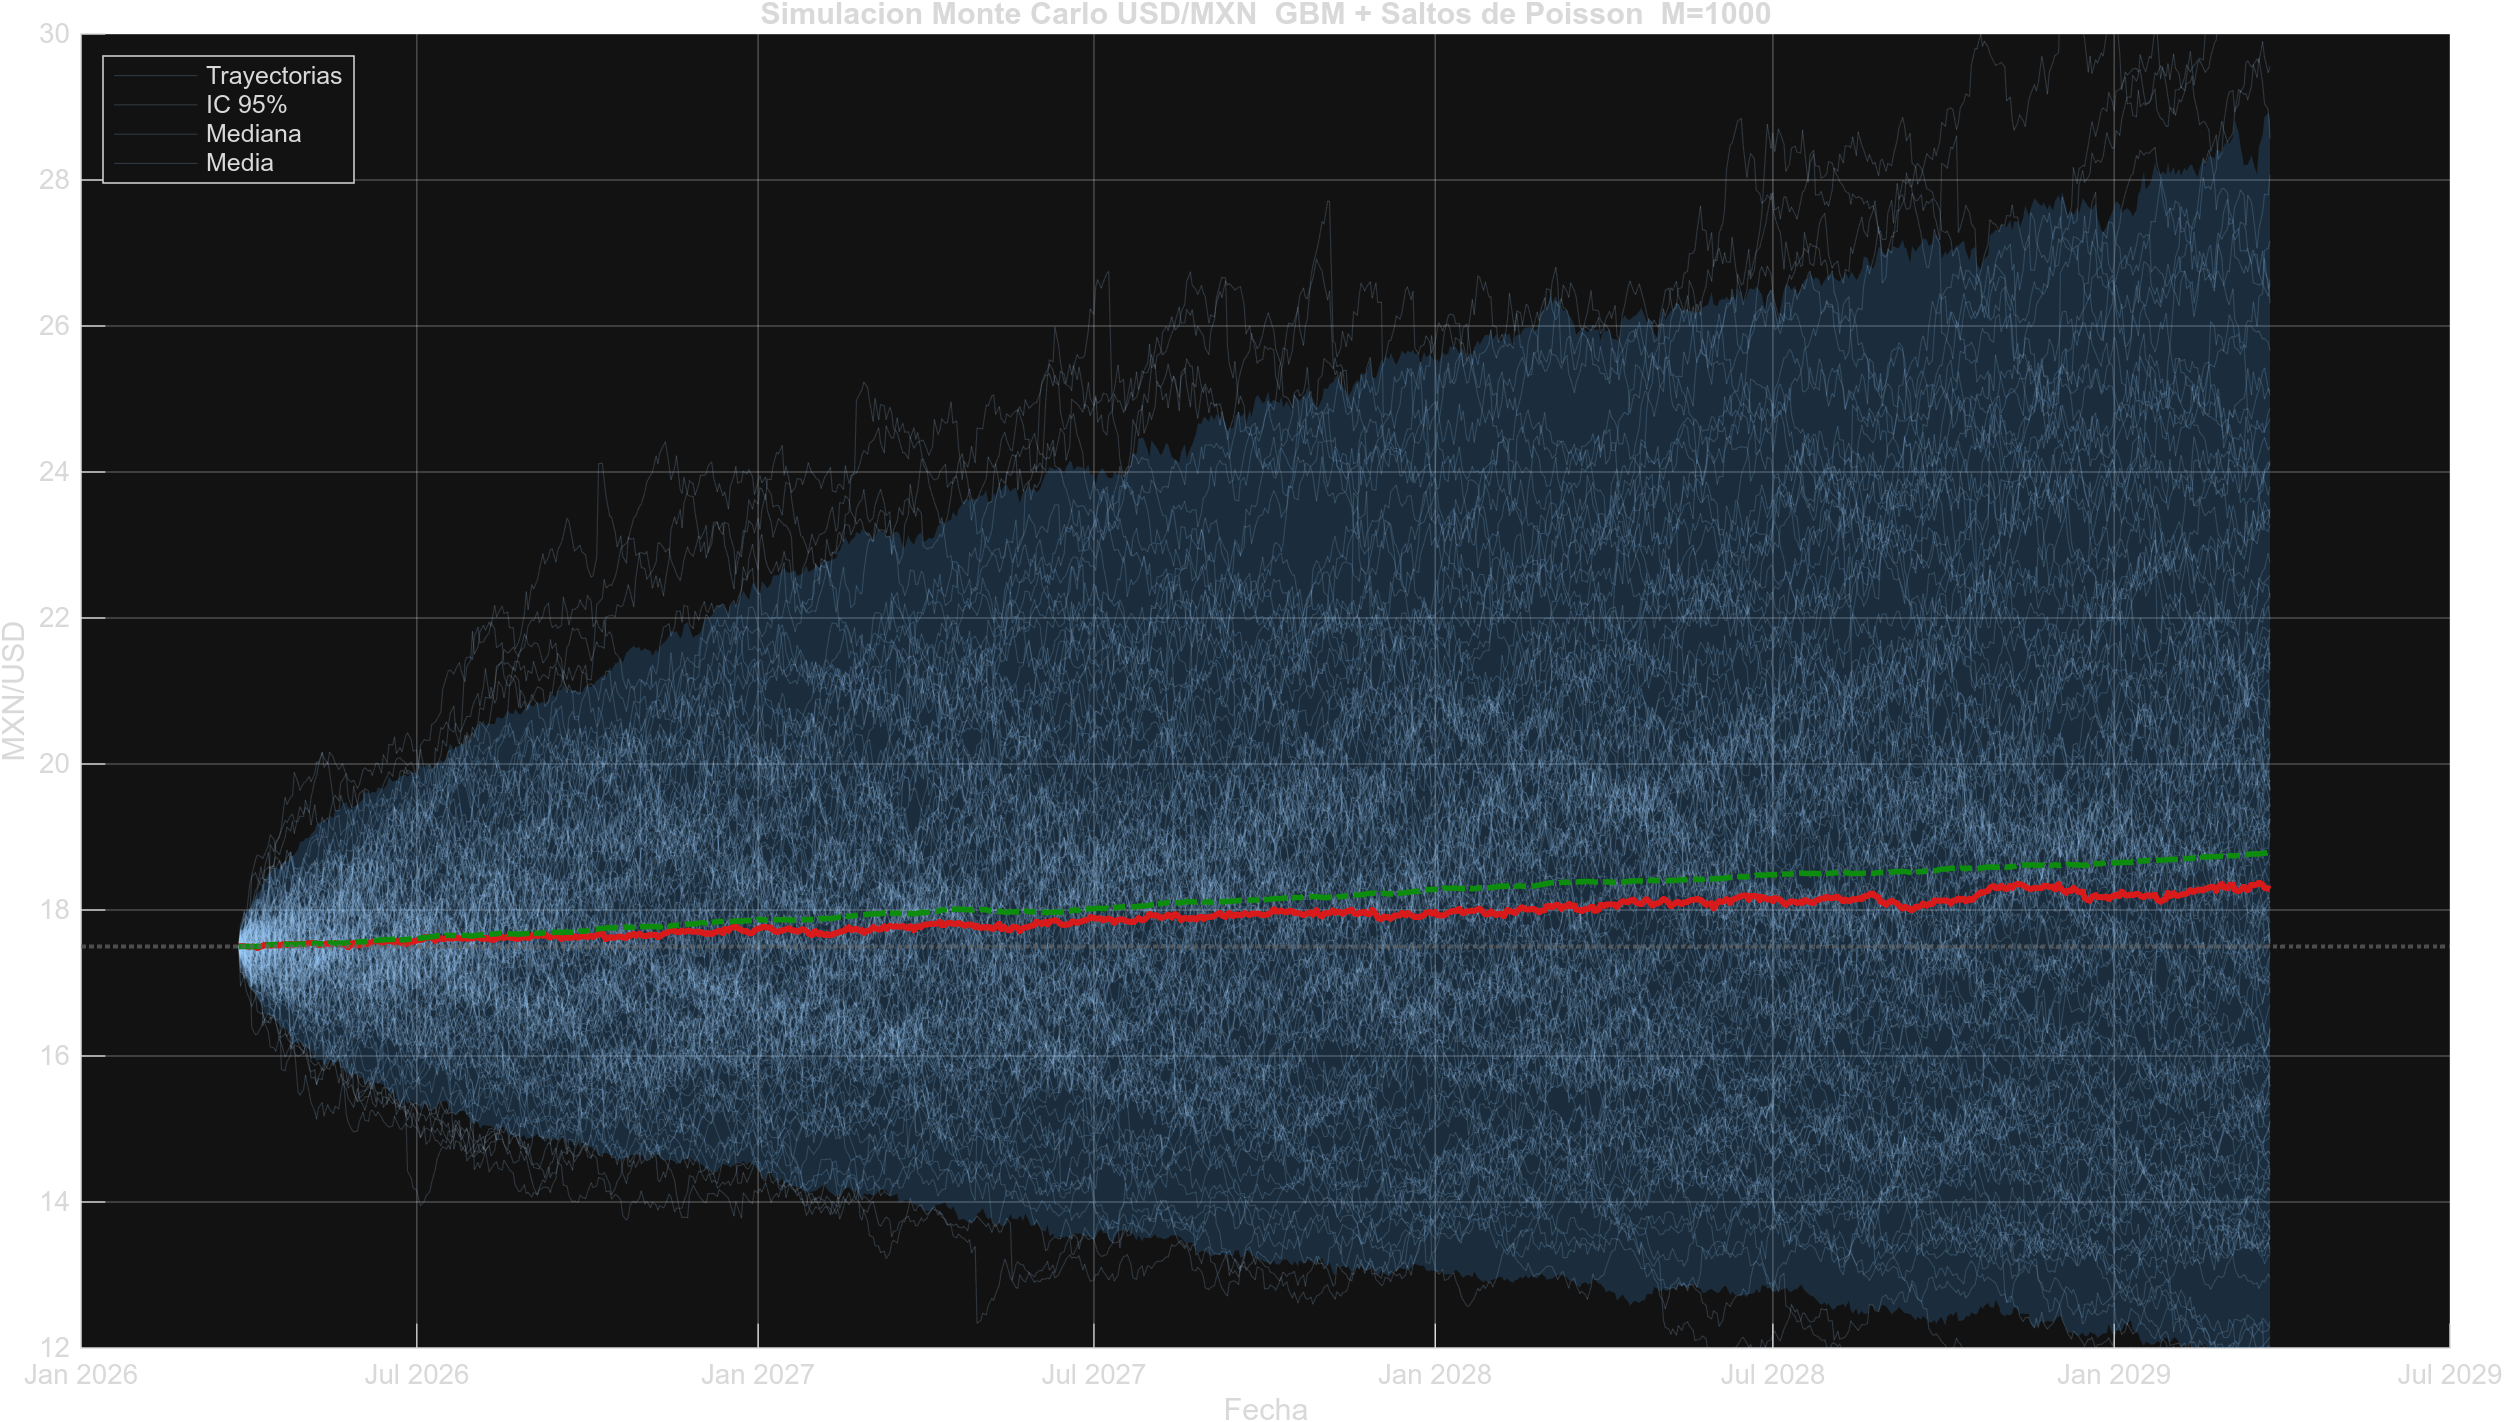
\includegraphics[width=\linewidth]{outputs/usdmxn_trayectorias.png}
        \caption{Trayectorias Monte Carlo con IC~95\% y 80\%}
    \end{subfigure}
    \hfill
    \begin{subfigure}[b]{0.50\textwidth}
        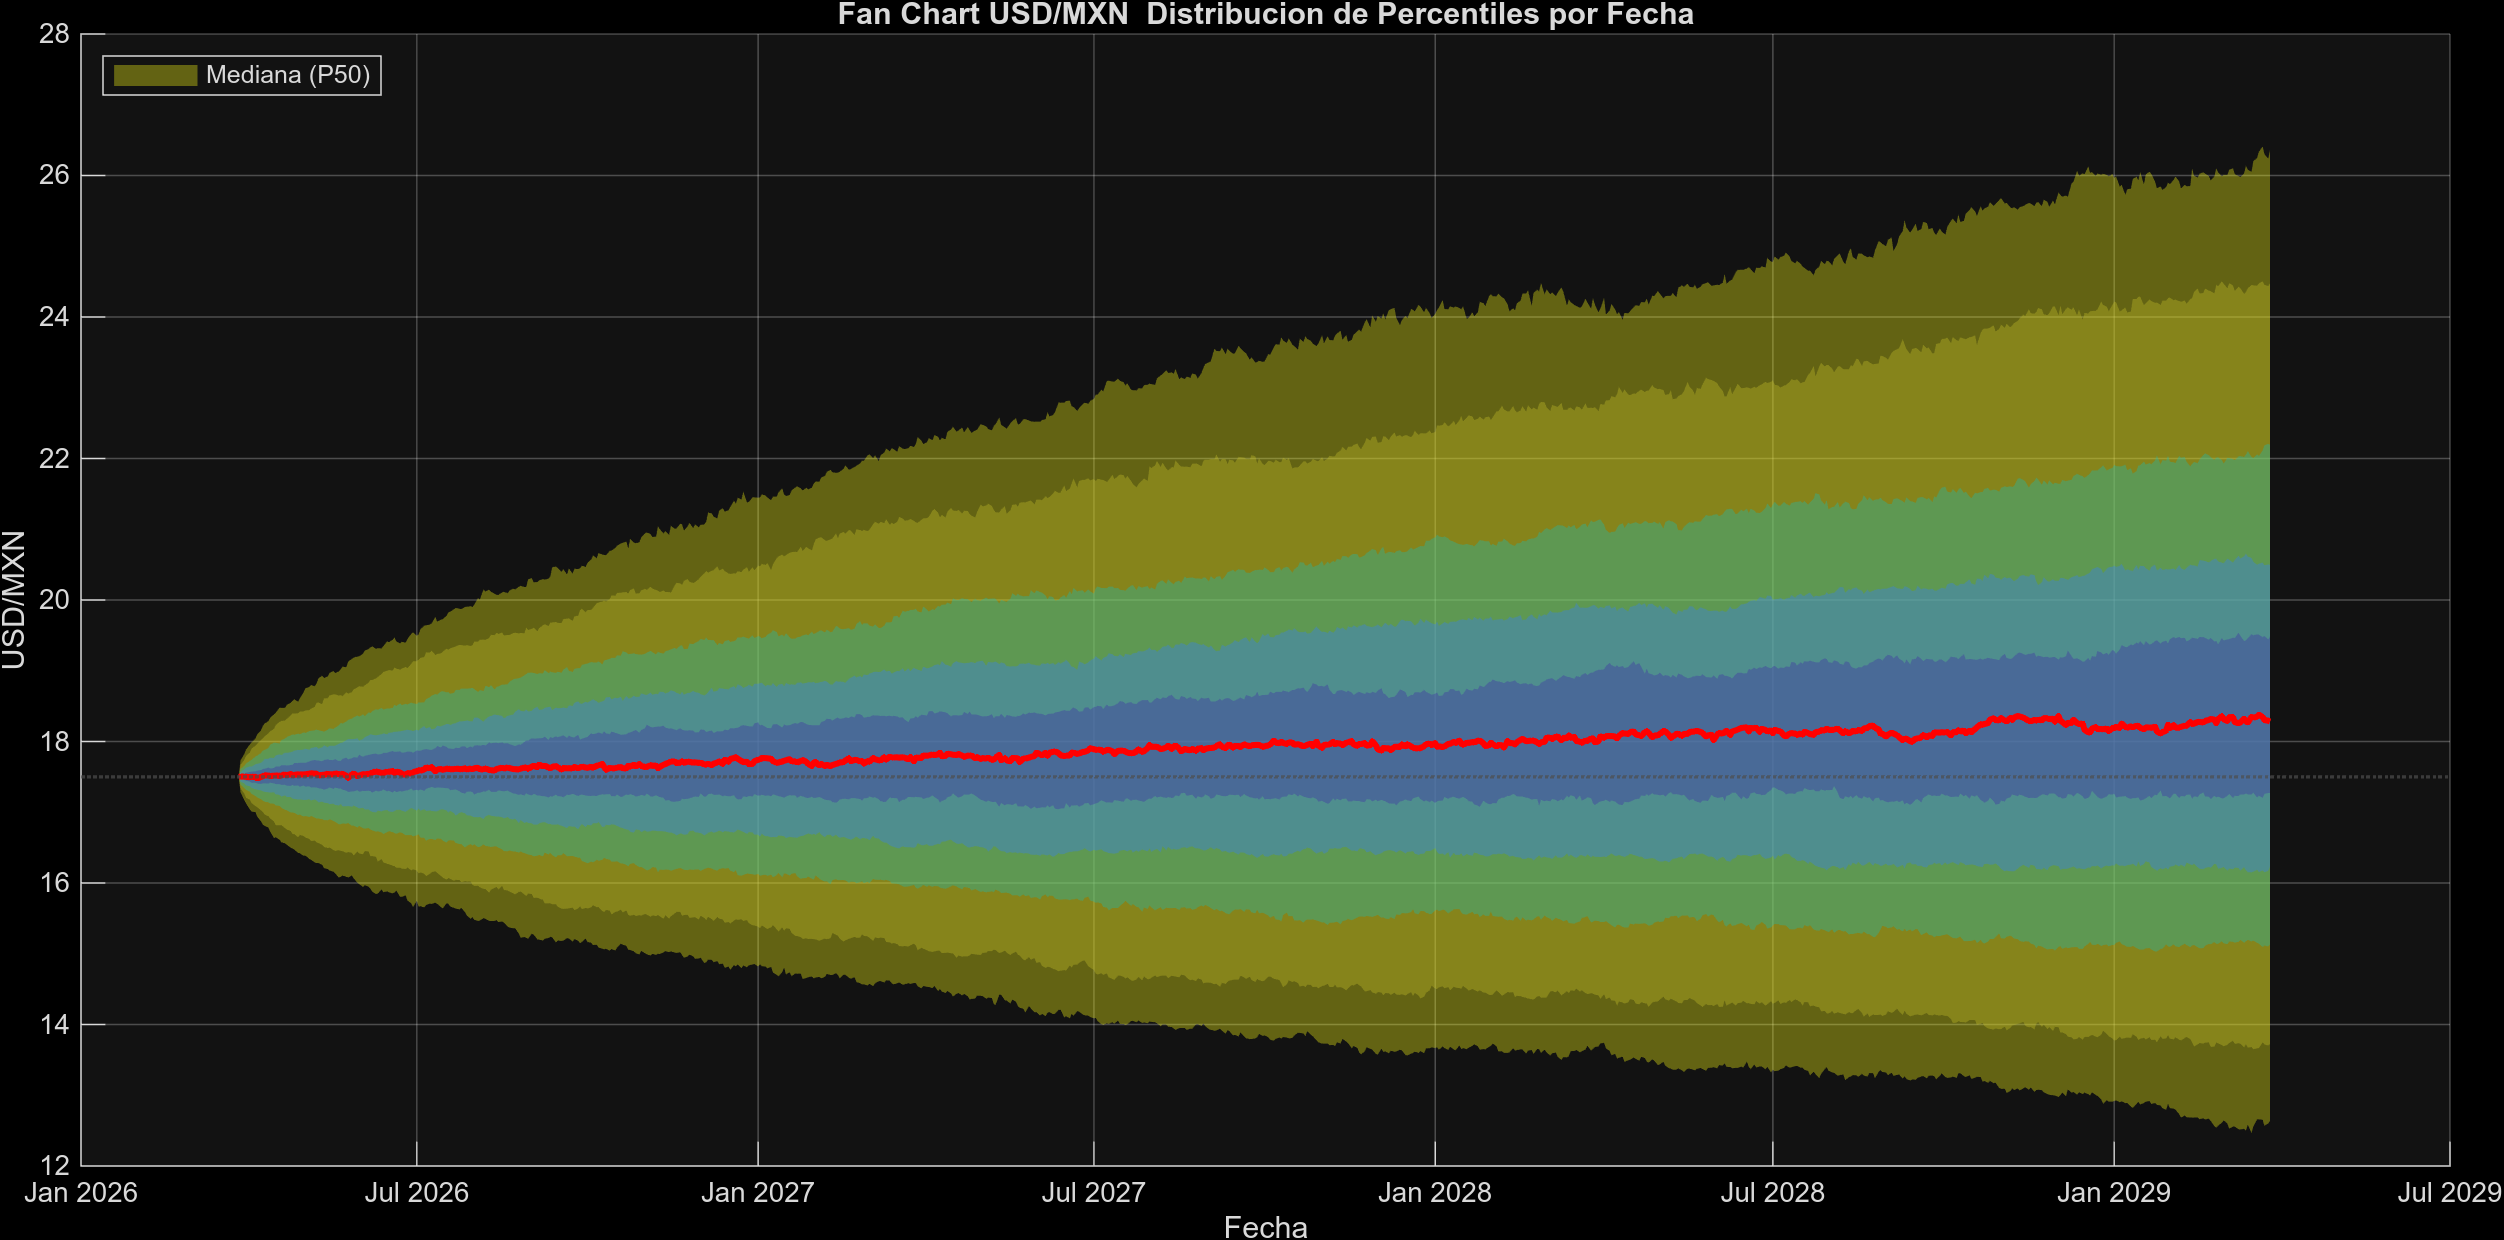
\includegraphics[width=\linewidth]{outputs/usdmxn_fanchart.png}
        \caption{Fan chart: bandas de percentiles P5--P95}
    \end{subfigure}
    \caption{Resultados gráficos de la simulación (\texttt{trial1.m})}
    \label{fig:resultados}
\end{figure}

\begin{figure}[H]
    \centering
    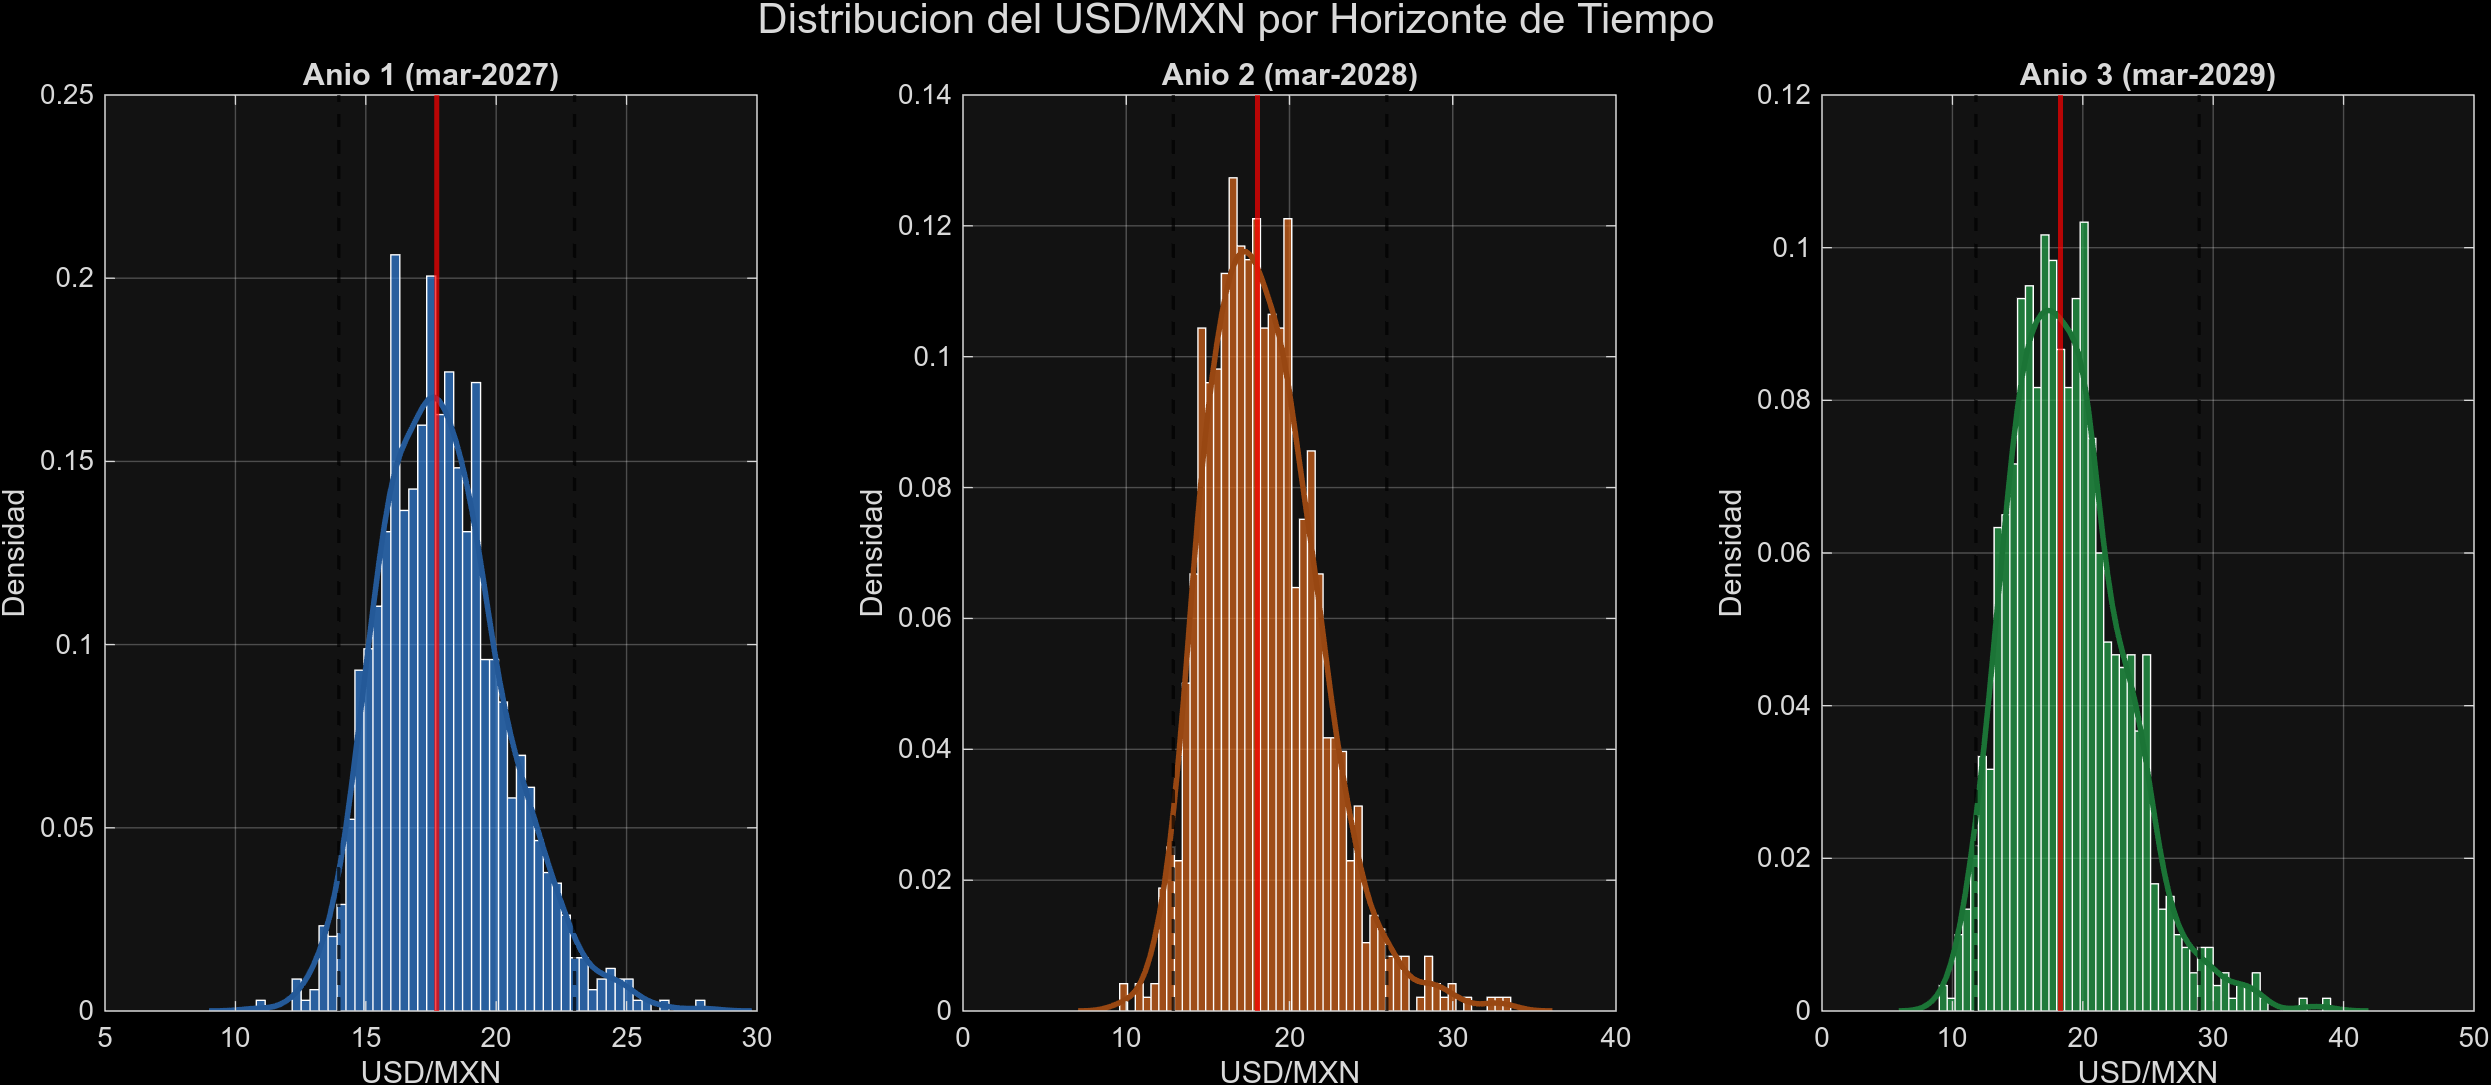
\includegraphics[width=0.95\linewidth]{outputs/usdmxn_distribuciones.png}
    \caption{Distribución marginal del USD/MXN al año 1, 2 y 3 con KDE}
    \label{fig:distribuciones}
\end{figure}

% =========================================================================
\section*{6. Resumen Ejecutivo de Parámetros}
% =========================================================================

\begin{center}
\begin{tabular}{@{}llll@{}}
\toprule
\textbf{Categoría} & \textbf{Parámetro} & \textbf{Símbolo} & \textbf{Valor} \\
\midrule
\multirow{5}{*}{Monte Carlo}
    & Trayectorias           & $M$           & 1\,000 \\
    & Horizonte              & $T$           & 3 años \\
    & Paso temporal          & $\Delta t$    & $1/252$ \\
    & Pasos totales          & $N$           & 756 \\
    & Semilla                & ---           & 42 \\
\midrule
\multirow{3}{*}{GBM}
    & Tipo de cambio inicial & $S_0$         & 17.50 MXN/USD \\
    & Deriva anual           & $\mu$         & 2.5\,\% \\
    & Volatilidad anual      & $\sigma$      & 11.5\,\% \\
\midrule
\multirow{4}{*}{Saltos (Merton)}
    & Intensidad             & $\lambda_j$   & 3.0 saltos/año \\
    & Tamaño medio (log)     & $\mu_j$       & $-0.010$ \\
    & Dispersión del salto   & $\sigma_j$    & $0.030$ \\
    & Deriva corregida       & $\mu^*$       & $\approx 5.352\,\%$ \\
\midrule
\multirow{2}{*}{Confianza}
    & Nivel IC               & $1-\alpha$    & 95\,\% \\
    & Percentiles fan chart  & ---           & P5 a P95 (5 bandas) \\
\bottomrule
\end{tabular}
\end{center}

% ---- PIE DE PÁGINA FINAL ----
\vfill
\begin{center}
{\color{anahuac}\rule{\linewidth}{0.5pt}}\\[0.2cm]
\small
\textbf{Prof.~D.Sc.~Aboud Barsekh-Onji, M.EEng., M.C.M.}\\
Facultad de Ingeniería, Universidad Anáhuac México \textbar{}
DIRCOM, Embajada de Qatar en México\\
\href{mailto:aboud.barsekh@anahuac.mx}{aboud.barsekh@anahuac.mx} \textbar{}
ORCID:~0009-0004-5440-8092
\end{center}

\end{document}
